%!TEX root = main.tex
\chapter{面向神威超算系统的大规模并行优化方法} % (fold)
\label{cha:面向神威超算系统的大规模并行优化方法}

\section{神威超算系统概述} % (fold)
\label{sec:神威超算系统概述}

\subsection{神威超算软硬件环境}
\label{sub:神威超算软硬件环境}
太湖之光超级计算机系统是“国家863”重大科研专项的研究成果,是第一台全部采用国产处理器、也是世界上首台峰值性能超过100PFlops的超级计算机。太湖之光自2016年6月起,已经连续获得4次Top500排名冠军。表\ref{tb:sunwaystat}描述了太湖之光超级计算机系统参数。全机峰值性能为125PFlops,内存总容量为1.31PB,缓存总带宽为5591TB/s,网络链路传输带宽为14GB/s,磁盘容量为20PB,IO聚合带宽为341GB/s,性能功耗比为6.05GFlops/W。


% Please add the following required packages to your document preamble:
% \usepackage{graphicx}
\begin{table}[ht]
\centering
\caption{太湖之光超级计算机系统基础参数。}
\label{tb:sunwaystat}
\resizebox{\textwidth}{!}{%
\begin{tabular}{ccccccc}
\hline
峰值性能      & 内存总容量  & 缓存总带宽    & 网络带宽   & 磁盘容量 & IO聚合带宽  & 性能功耗比        \\ \hline
125PFlops & 1.31PB & 5591TB/s & 14GB/s & 20PB & 341GB/s & 6.05GFlops/W \\ \hline
\end{tabular}%
}
\end{table}

太湖之光有高速运算系统、高速互联网络和网络存储系统组成(如图\ref{fig:sunwayarch}所示)。高速运算系统由40960个节点组成。其中每4个节点组成一个计算板,每64个计算板以全连接的方式组成一个超节点。4个超节点构成一个机柜,40个机柜则集成了峰值性能超过125PFlops的神威超算。神威超算采用Lustre并行文件系统,通过高速互联网络与运算系统连接。神威超算的计算节点通过InfiniBand网络相连,节点间双向传输带宽为14GB/s,全网双向带宽为56GB/s,超节点内使用全连接网络,超节点间则使用两层胖树结构网络相连。

\begin{figure}[ht]
\centering
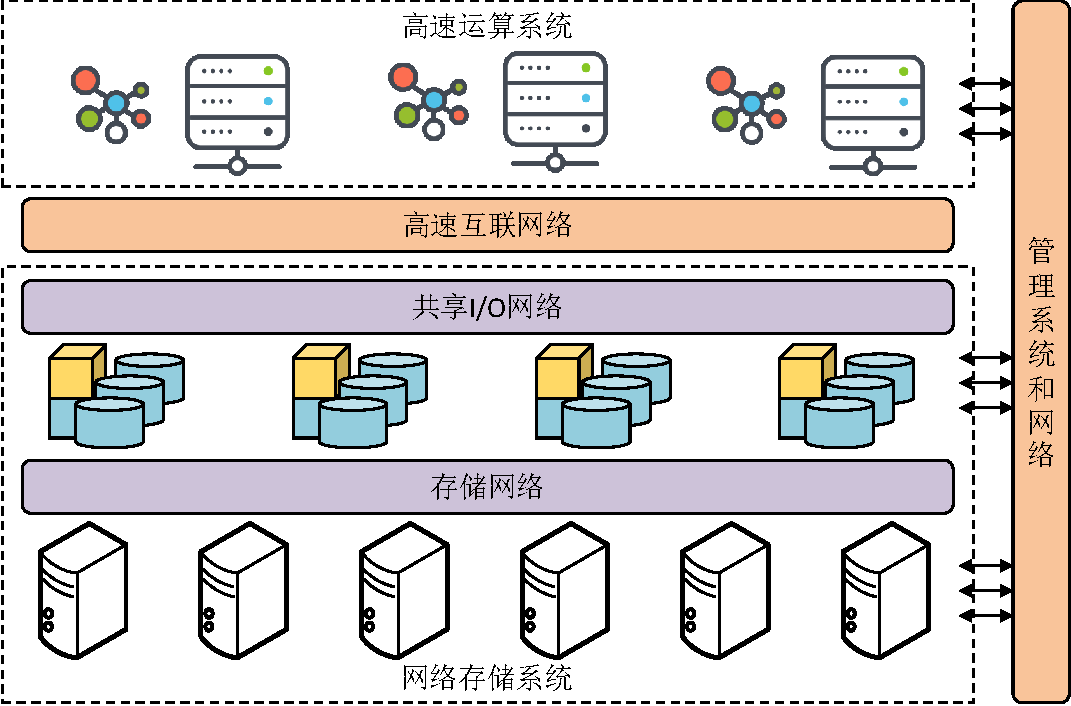
\includegraphics[width=.9\columnwidth]{太湖之光系统架构图-crop.pdf}
\caption{太湖之光超算系统架构图。}
\label{fig:sunwayarch}
\end{figure}

太湖之光的软件系统架构如图\ref{fig:sunwaysofts}所示,包含底层的并行操作系统环境与高性能存储管理系统、国产众核CPU基础软件、并行语言及编译环境、并行开发环境与并行应用。作为主要支持大型科学计算的超级计算机,太湖之光支持C/C++和Fortran等常用编程语言,并提供了完备的基础函数库(如C标准库、加速线程库、数学库等),且支持了循环级向量化。

\begin{figure}[ht]
\centering
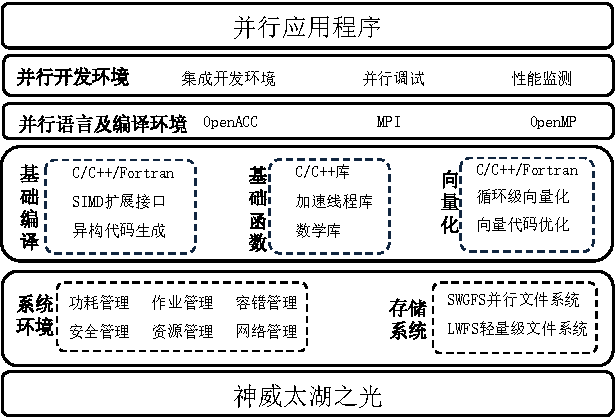
\includegraphics[width=.8\columnwidth]{太湖之光软件系统-crop.pdf}
\caption{太湖之光软件系统架构图。}
\label{fig:sunwaysofts}
\end{figure}

\subsection{神威超算与其他领先超算的比较}

太湖之光超级计算机采用了与传统超算(纯CPU、CPU+GPU、CPU+MIC等)完全迥异的架构——申威26010架构,每个节点包含4个主核和256个从核。与世界上其他领先超算相比,神威超算的峰值计算性能、持续计算性能、节点数和计算核心数都大幅领先,分别是排名第二的天河二号的2.3、2.7、2.56、3.4倍(如表\ref{tb:system-comp}所示)。然而与计算能力相比,神威超算在内存方面在并没有太大的优势,其总内存容量为1,310TB,略低于天河二号的1,375TB。由于神威超算节点数目众多,因此每个节点可用内存也低于其他超算。此外,神威超算单节点的内存带宽仅为136GB/s,而领先的Intel KNL 7250芯片的内存带宽为562GB/s,NVIDIA P100 GPU的内存带宽为732GB/s。因此神威超算的优势在于强大的计算能力和众多的计算节点。而对于访存受限的应用,由于神威超算的内存带宽较低,其优化面临着更严峻的挑战。

\begin{table*}[ht]
\footnotesize
\caption{太湖之光超算系统与其他超算系统的比较。}
\label{tb:system-comp}
\resizebox{\textwidth}{!}{%
\begin{tabular}{ccccccccccc}
\hline\hline
  超算系统 & 峰值性能 & 持续性能 & 计算节点数 & 计算核心数 & 处理器架构 & 内存 & 能耗\\
  & (Pflops) & (Pflops) &&&& size (TB) & (kW)\\\hline
  太湖之光 & 125  & 93 & 40,960 & 10,649,600 & 4主核 & 1,310 & 15,371 \\
  & & & & & +256从核 \\\hline
  天河二号 & 55 & 34 & 16,000 & 3,120,000 & 2个12核CPUs & 1,375 & 17,808\\
  & & & & & +3个57核 MICs \\\hline
  Titan & 27 & 18 & 18,688 & 560,640 & 1个16核CPU & 710 & 8,209 \\
  & & & & &+ K20x GPU \\\hline
  Sequoia & 20 & 17 & 98,304 & 1,572,864 & 16核CPU & 1,572 & 7,890 \\\hline
  Cori & 28 & 14 & 9,152 & 622,336 & 68核CPU & 878 & 3,939\\\hline
\hline
\end{tabular}
}
\end{table*}

综上所述,神威超算超大规模计算能力、申威26010芯片独特的片上异构众核架构在扩展性、访存效率等角度为应用提供了巨大的优化空间。因此,本文工作将其作为主要研究平台,从内存带宽、从核计算、扩展性、通信和IO和应用算法优化多方面出发,为天然大地震模拟和人工地震勘探的研究提供高性能计算支持。

\section{多层级并行设计方案}
\label{sec:多层级并行设计方案}

\subsection{并行任务划分基本原则}

当地球物理勘探应用需要处理较大区域的地震数据时,单节点计算机无法满足应用软件所需的内存和计算需求,并行计算机系统应运而生。例如,在一次典型的石油勘探中,勘探的区域通常为$100km\times100km\times60km$,空间分辨率为$20m$,在不考虑边界的情况下,计算网格的格点数为$7.5\times10^9$。石油物探应用通常使用单精度浮点数表示每个格点,因此每个表示完成勘探区域的数组的大小约为$3\times10^10$字节,即30TB。这远远超出了单个节点内存上限。因此,我们需要对勘探区域进行进一步区域分解。

传统并行计算通常采用单指令多数据(SIMD)并行模式将统一的大规模数据分解成若干小数据,并将其分配到不同的节点参与计算。在同构集群中,常用的并行策略包括纯MPI并行、MPI-OpenMP混合并行;在异构的GPU集群中,通常采用MPI-GPU并行方式。

神威超算拥有超大规模的40,960个计算节点,计算节点间通过Infinite Band网络相连。每个节点包含4个核组,每个核组又由一个主核和64个从核组成。核组间可以通过MPI进行进程级别的通信,从核间既可以通过共享主存交换数据,还可以通过神威架构独有的寄存器通信特性进行通信。可以与传统异构集群相比,神威超算的不同处理单元层次更加鲜明,不同处理单元的计算和通信方式也各不相同,这为如何将科学应用进行合适的任务划分以高效扩展到神威超算的所有计算节点提供了巨大的探索空间。

任务划分的基本思想是将完整的大计算任务分解成若干小任务并派发到不同的节点并行计算。在多节点计算时,节点间的数据的交换通过网络或者存储来完成,其效率一般会低于节点内的内存数据交换效率。计算完毕后,将结果汇集到主计算节点而形成最终计算结果。并行任务划分决定着通信方式、通信量和通信粒度,因此良好的任务划分是大规模并行计算高效运行的关键。并行任务划分通常遵循以下基本原则:
\begin{itemize}
  \item 分配给每个计算节点的任务尽量均衡。一般的并行计算机系统采用相同的节点连接而成,每个节点的处理能力相当,如果出现某个节点需执行大量任务,则必要会使其他节点闲置等待,造成负载不均衡现象,影响整体运算性能。
  \item 尽量降低节点间通信开销。将一个完整的大问题分解成若干小问题并让不同计算节点计算完成的过程中,难免需要引入节点间额外的数据交换开销。在小规模并行计算中,通信不会成为主要的应用的瓶颈,但是当并行规模达到成千上万甚至十万百万量级时,通信的开销将变得不可忽略,有限的通信带宽与随之而来的通信延迟将极大降低通信的效率,此时通信甚至会成为主要的瓶颈。因此,采取适当的划分方法降低节点间通信的开销能够很好地缓解这个问题。此外,在大规模的并行应用中,还应该尽可能避免大量集合通信。集合通信要求不同进程在程序运算时特定时间点进行同步,而不同进程几乎很难在同一时刻到达集合通信点,会出现先到达的进程等待的现象,而先到达的进程又有可能在下次集合通信点晚点到达,导致不同进程交叉等待,降低了超算不同资源的利用效率。使用异步的非集合通信能够有效地避免这个困扰。
  \item 充分利用寄存器通信。申威处理器寄存器通信特性为从核间的数据交互提供了高效的通信手段。使用寄存器通信,从核间的数据交互无需通过共享主存来完成,有利于降低DMA数据传输负担,节约DMA数据传输带宽。
\end{itemize}

在遵循上述原则的基础上,本研究结合地震模拟的真实应用场景,提出了多层级并行任务划分方案。该方案不仅适用于地震模拟应用,还适用于其他大规模规整网格的基于$Stencil$计算的科学问题。

\subsection{多层级并行任务划分}

本小节首先介绍大规模$Stencil$运算的二维区域划分方法,该思想可以灵活扩展到三维$Stencil$区域划分,这将作为下文多层级并行任务划分的基础。

图\ref{fig:2ddecomposition}为二维MPI区域划分与一维从核计算划分示例。如图\ref{fig:2ddecomposition}所示,将完整的地震波传播波场按照不同颜色划分成四块,其中白色表示边界,也可表示Halo区域。每一个子波场派发给不同的计算核组(在使用神威超算大内存的情况下,也可以使用整个CPU替代四个核组),四个核组独立更新子波场,并在需要时更新Halo区域。在单核组处理中,我们调用64个从核加速运算。64个从核也可以按照不同的排列方式参与运算,不同的排列方式将影响数据从主存传输到从核LDM的开销以及不同从核间寄存器通信的开销。按照第\ref{sec:最小DMA数据传输方案}节的推导,此处从核使用一维排列方式即可实现高效的数据传输。

\begin{figure}[th]
  \centering
  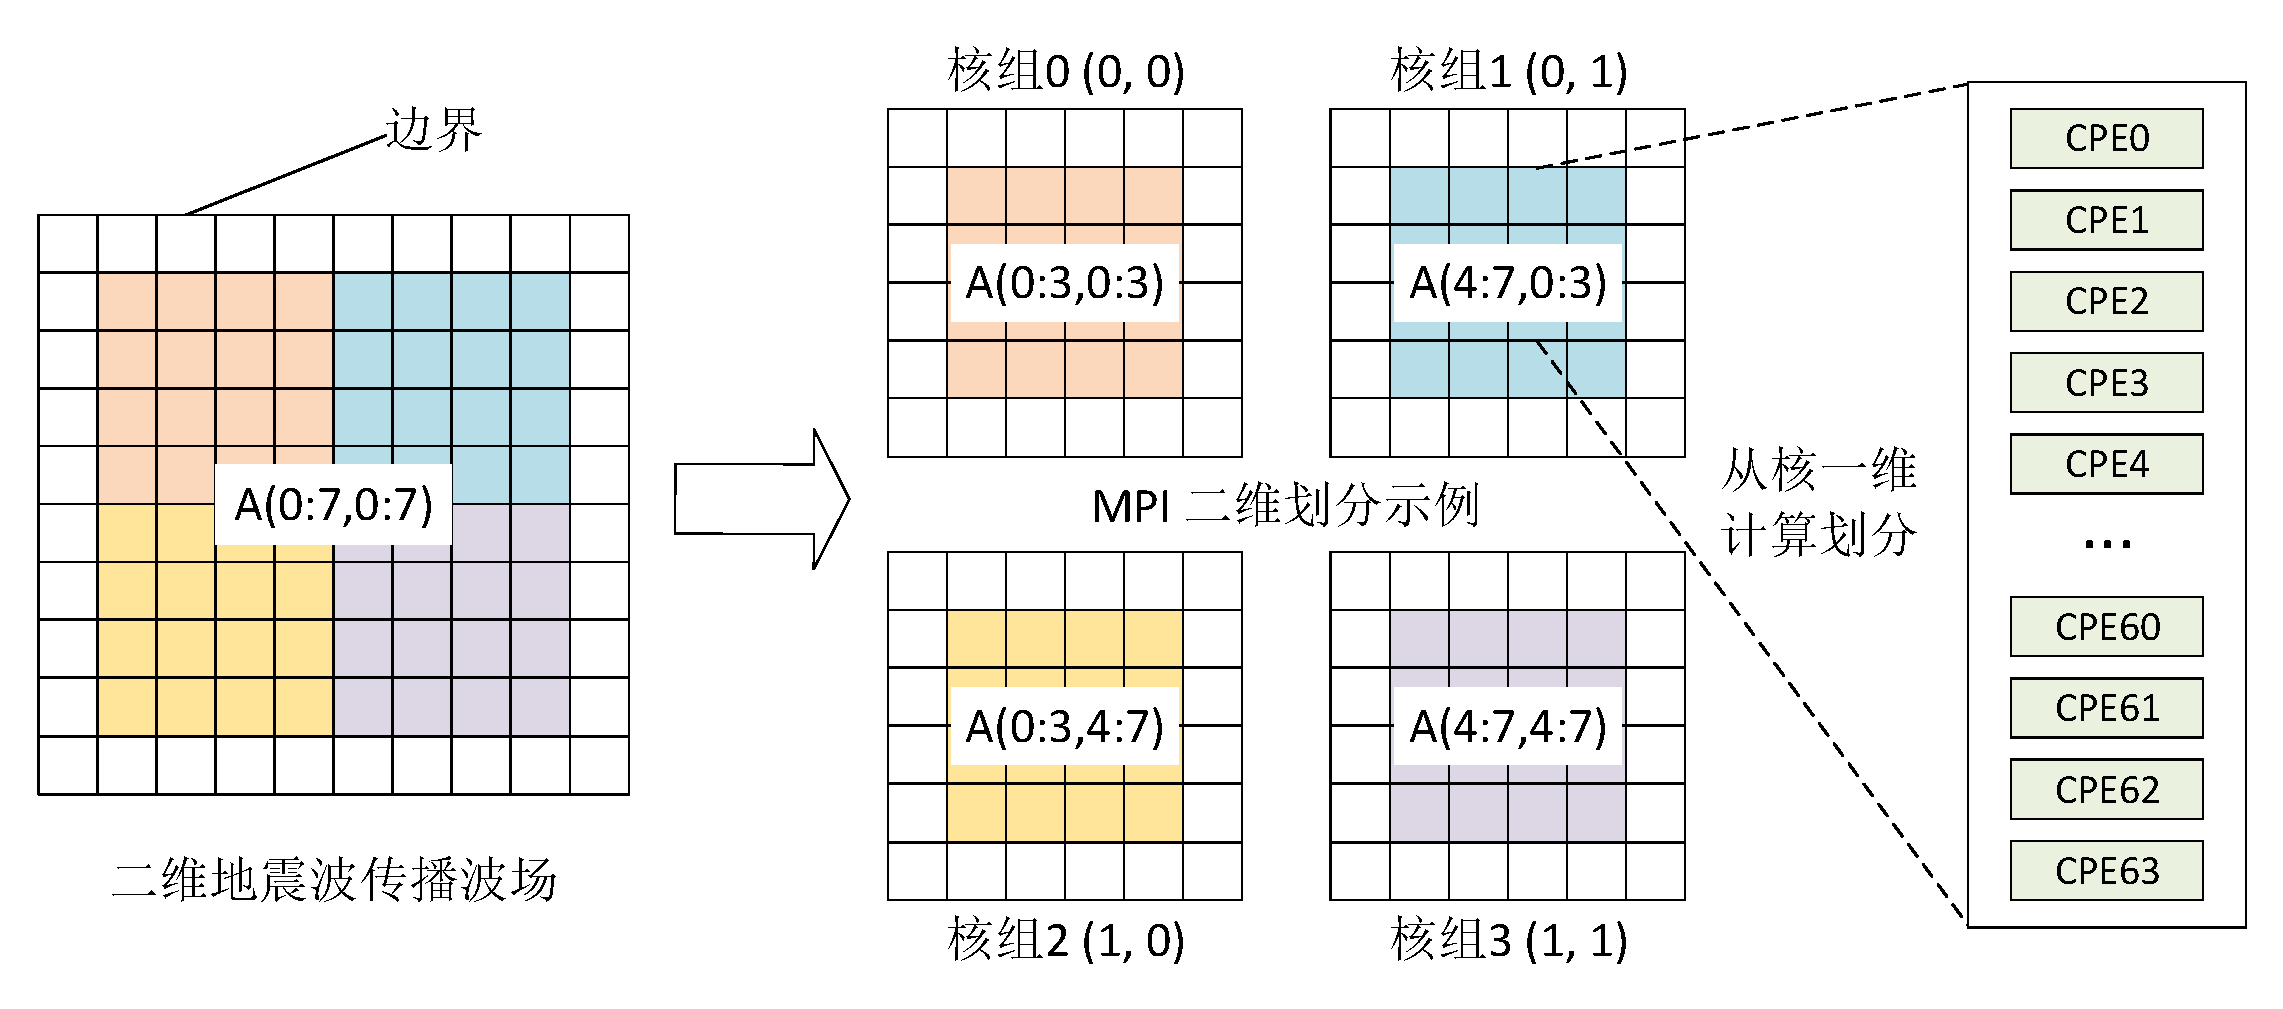
\includegraphics[width=1.0\columnwidth]{2ddecomposition.pdf}
  \caption{二维MPI区域划分与一维从核计算划分示例。}
  \label{fig:2ddecomposition}
\end{figure}

在三维弹性波正演过程中,更新速度和应力的核函数(kernel function)包括20-50个覆盖完整区域并设计读写的变量数组。许多适用于X86平台或GPU平台的优化技术,如3.5D blocking等方案\citep {nguyen20103},都由于极高的内存容量要求而在申威芯片上变得不切实际。本文工作通过深入剖析神威超算的架构特点,从核组间、核组内、从核间、从核内等多个维度出发,提出了多层级并行设计方案(如图~\ref{fig:dd}所示),能高效地将地震波传播模块扩展到160,000核组,达到接近线性的扩展性,同时最大限度地降低了相关内存成本。多层级并行设计方案包括以下四部分。

\begin{figure}[ht]
\centering
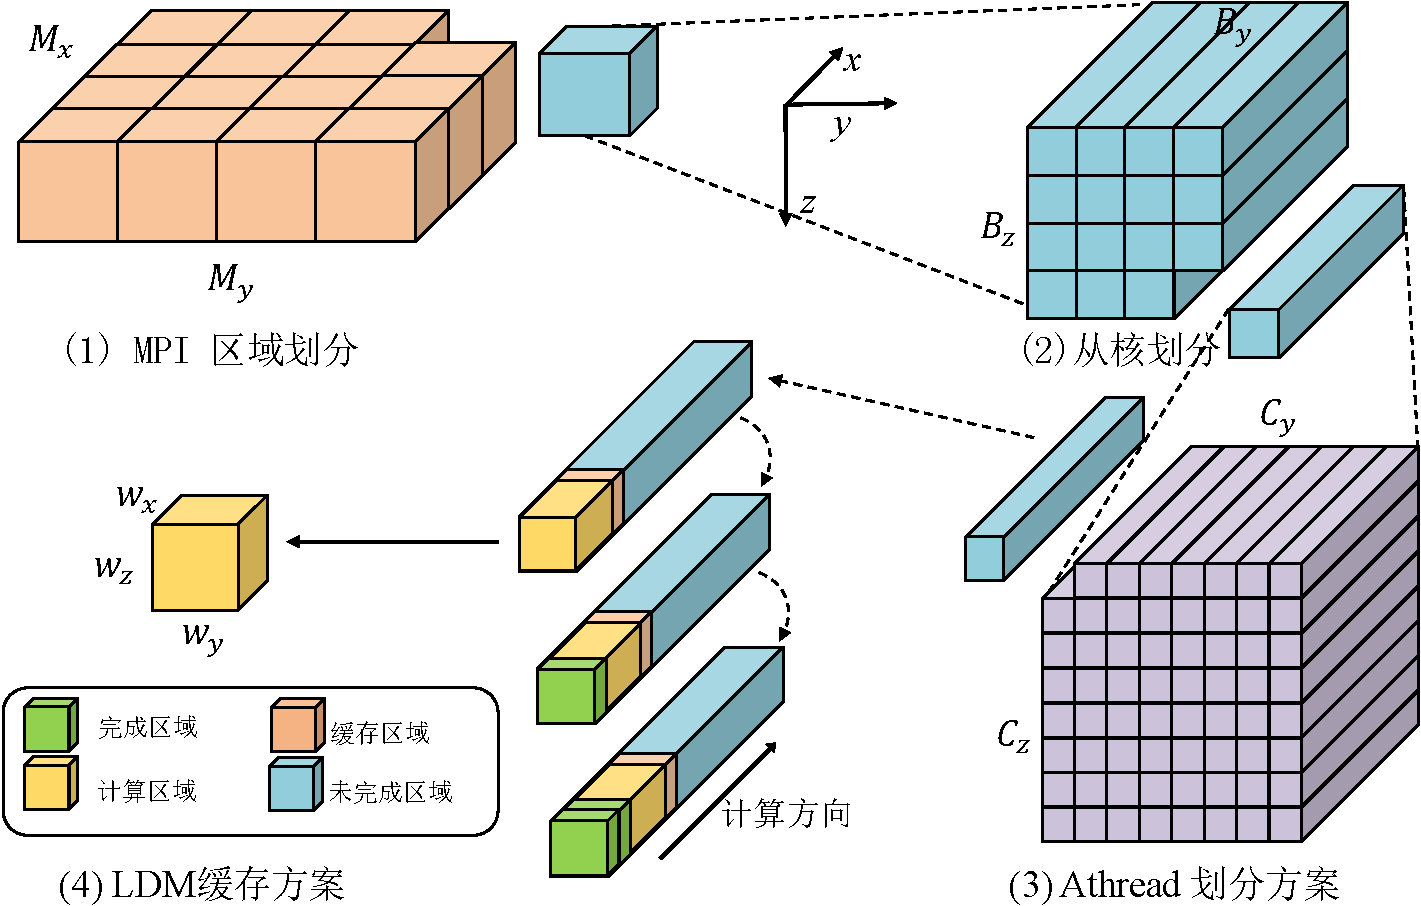
\includegraphics[width=0.9\columnwidth]{blocking-crop.pdf}
\caption{多层级并行设计方案:(1)MPI进程的二维分解; (2)每个核组内分解;(3)Athreads的二维分解;(4)LDM缓存方案。}
\label{fig:dd}
\end{figure}

基于核组间的二维区域分解。在三维地震模拟中,通常将$ z $轴(垂直方向)作为最快轴,将$ y $轴作为第二快轴,并将$ x $轴作为最慢的轴。在典型的地震模拟情景中,$ x $和$ y $(一般是几百公里)的尺寸通常比$ z $(一般是几十公里)大得多。因此在第一级划分中,为了尽量减少进程之间的通信以及增大DMA传输带宽,本文工作将地震模拟区域沿$x$和$y$轴划分为$ M_x $ $ M_y $个不同的分区,每个分区对应特定的MPI进程并分配给独立的核组,在AWP-ODC\citep{cui2010scalable}计算与通信重叠的基础上,本文工作还包括了许多针对神威特殊架构的优化,如基于从核的内存拷贝。在极端情况下,基于核组间二维区域分解可将地震传播模块以97\%的效率扩展到神威超算整机,即160,000(400×400)个MPI进程。

基于核组内的二维区域分解。每个核组的内存为8GB,但每个从核LDM高速缓存只有64KB。第一级划分后的区域需要经过再划分以确立每个从核的工作任何。因此本文工作将核组内的数据沿着$ y-z $方向进行二维区域分解(第二级划分)。划分后的每一块的数据能够通过DMA传输到每个从核的LDM高速缓存中并参与计算。每个从核依次遍历所有分块,完成全部计算。

基于从核间的二维数据分解。申威架构中,高效的从核计算需要依托于高效的数据访问,因此必须将计算所需的数据提前传输到每个从核64KB的LDM高速缓存中。使用从核计算有限差分,每个核组中64个从核不同的逻辑排列方式对应着主存中不同的数据范围以及不同的DMA数据传输总量。本文工作中从核按照$y-z$排列,并对数据进行划分。每个从核使用Athread线程沿着$ x $方向迭代,以实现不同线程高效的数据访问和DMA数据传输。

基于从核内的一维数据分解。每个从核使用DMA操作将合适大小的计算区域,包括中心部分和Halo区域加载到LDM中参与运算。为了提高数据复用率和DMA传输效率,DMA操作在首次加载完毕后沿着$x$轴方向移动,每次加载一个$y-z$平面。由于$x$轴是慢轴,加载$y-z$平面能最大限度的利用数据在内存中的连续性,提升DMA传输效率。此外,不同从核的DMA数据传输虽然共享内存带宽,但从核间的DMA操作与计算过程却是异步的,能实现计算通信重叠,进一步提升效率。


\section{大规模并行通信优化方案}

当并行规模扩展到上万进程或者几十万进程时,应用的整体通信总量、通信链、延迟也随之增大,应用的热点会逐渐从计算转移到通信,通信开销甚至会成为整体应用的主要瓶颈。大规模并行通信优化的策略与第\ref{cha:面向申威异构众核处理器的并行优化方法}章的内存性能优化策略类似,也从三方面出发:减少通信总量、增大通信带宽与计算通信重叠。

\subsection{计算和通信重叠}

计算和通信分别占用了不同的资源,两者理论上可以并行执行以缩短相互计算和通信相互等待的时间。在同步MPI通信模型中,当前进程的速度子区域更新后需要将边界发送给邻居进程,同时也需要从邻居进程接收边界。通信完毕后才能执行应力的更新。同步的MPI通信模型在任意时刻只有计算或者通信单一资源被利用,效率不高。本研究采用异步MPI通信模型,通过添加两层虚拟网格实现计算和通信重叠。

图\ref{fig:2ddecomposition}所示的区域划分中,每个MPI进程需要在每个迭代步结束之后统一执行Halo区域的更新,这涉及到同步的MPI操作,会导致不同的进程在不同的迭代步交叉等待。为了进一步提升整体性能,我们为每个MPI进程设计了Halo区域更新异步通信,如图\ref{fig:comp-comm-overlap}所示。

\begin{figure*}[ht]
    \centering
    \begin{subfigure}[b]{0.5\textwidth}
        \centering
        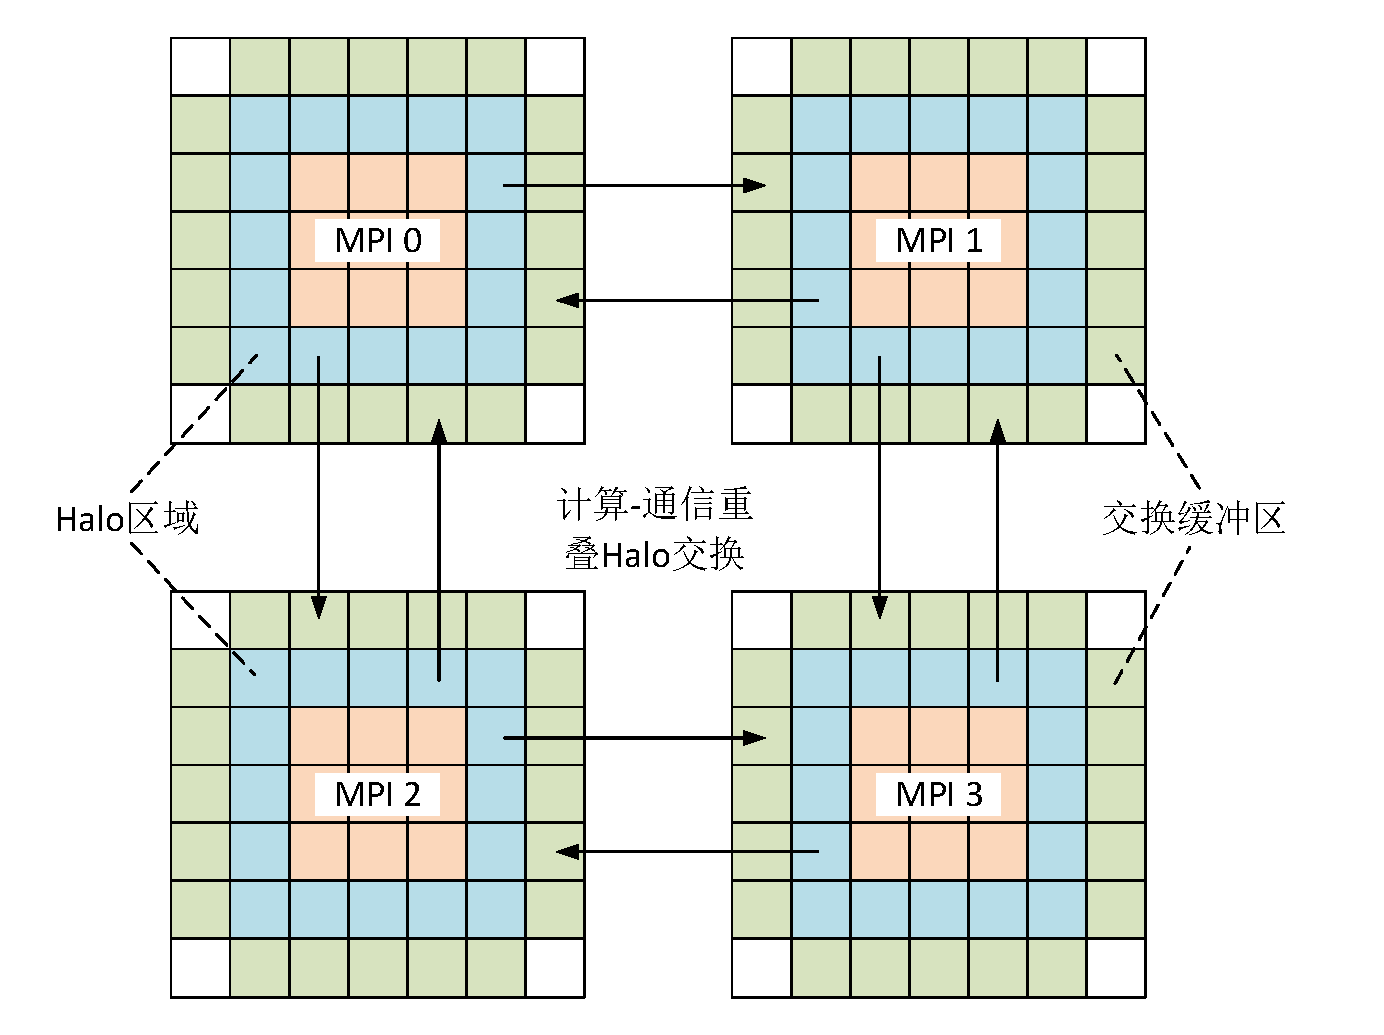
\includegraphics[height=2.5in]{comp-comm-overlap.pdf}
        \caption{计算与通信重叠MPI划分示例。}
        \label{fig:comp-comm-overlap}
    \end{subfigure}%
    ~
    \begin{subfigure}[b]{0.5\textwidth}
        \centering
        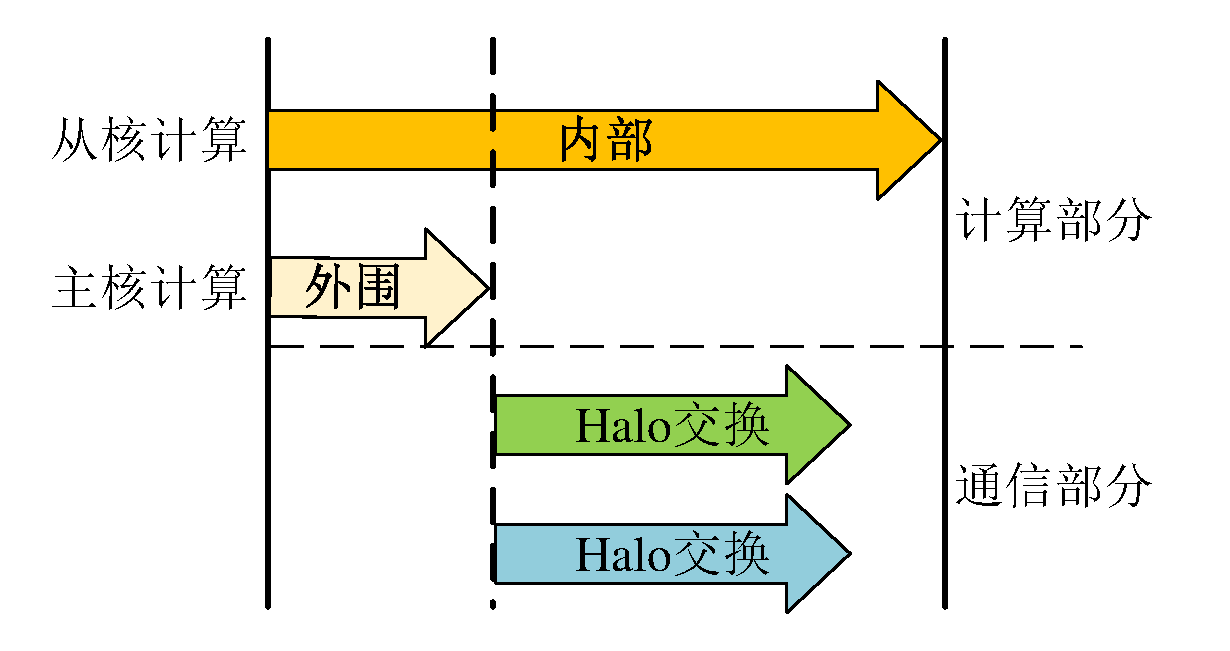
\includegraphics[height=2in]{overlappipe.pdf}
        \caption{计算与通信重叠运算时间示例。}
        \label{fig:overlappipe}
    \end{subfigure}
\end{figure*}

与图\ref{fig:2ddecomposition}相比,图\ref{fig:comp-comm-overlap}中每个核组处理的区域中包含内部主要计算部分、Halo区域和Halo交换缓冲区。按照以下步骤完成Halo区域交换的计算和通信重叠过程。%(如图\ref{fig:comp-comm-impl}所示)。

\begin{itemize}
  \item 每个MPI进程调用异步MPI通信接受接口($MPI\_Irecv$),接收发送给当前MPI进程的Halo数据,并将其存储在交换缓冲区中(绿色)。由于调用的是异步接口,主线程立即返回执行后续计算。
  \item 每个MPI进程首先计算子区域的Halo区域(蓝色),使用异步MPI接口($MPI\_Isend$)把Halo区域发送给当前进程邻接的四个(二维划分)或六个(三维划分)进程,待发送的Halo区域将被复制到MPI缓冲区中独立发送,此时该进程无需等待Halo区域发送完毕而继续执行后续计算。
  \item 每个MPI核组的从核对内部区域(红色)进行有限差分计算,更新波场。此时的计算上一步的MPI发送是异步并行的,实现了计算与通信重叠。
  \item 当需要更新下一个波场(别的变量)或者下一个迭代步时,调用MPI同步接口($MPI\_Waitall$),保证上述的发送和接收数据达到指定的目的地。值得注意的是,在进程发出异步发送Halo区域数据时,MPI的通信和后续的计算并行执行,因此在调用$MPI\_Waitall$接口时,Halo区域数据已部分到达或者完全到达,取决于通信和计算的开销比例(如图\ref{fig:overlappipe}所示)。
  \item 将交换数据缓冲区中的Halo数据复制到实际Halo区域,并进入下一个迭代步。
\end{itemize}

这种区域划分和及通信方式能够获得很好的可扩展性。首先,每个MPI进程分配到的区域大小是相同的,需要进行通信的Halo区域数据大小也完全相同,不会出现负载不均衡问题。其次,完整区域的更新由每个小区域的更新构成,无需进行全局通信操作。不管应用扩展到多大的规模,每个MPI进程只需要发送和接收与其邻接的四个或者六个进程的数据,即便出现不同进程运行速度不同,相距较远的进程间由于不需要数据通信不会相互等待。进程间运行速度不同只会影响邻接进程。另外邻居进程只有4-6个,影响很小。

\subsection{虚拟网格}

大规模正演的主要延迟来源于不同计算节点间的数据通信。在三维弹性波正演的每个迭代步中需要进行三个速度分量和六个应力分量的边界通信。根据第\ref{sec:多层级并行设计方案}的介绍,本研究对完整地震区域进行二维划分($x-y$方向),则通信发生在(1:nx, 1:ny, 1:NZ)子区域,其中nx、ny表示每个进程内x-y方向的范围,NZ表示完整区域的深度。二维划分下,每个进程(边界除外)需要与4个邻居交换9个变量的边界。对于13点的三维$Stencil$运算,计算每一个中心点需要索引该中心点的上下左右前后各2个格点,因此子区域的每个方向需要向外扩展两层虚拟网格(ghost cell)才能完成整个子区域的更新。这意味着需要更新大小为(1:nx, 1:ny, 1:NZ)的子区域需要大小为(-1:nx+2, -1:ny+2, 1:NZ)的网格输入。

更准确地说,在每个迭代步中,如果需要更新大小为(1:nx, 1:ny, 1:NZ)的速度子区域,则需要大小为(-1:nx+2, -1:ny+2, 1:NZ)的应力子区域。每个迭代步需要更新速度和应力,同理可得,更新大小为(1:nx, 1:ny, 1:NZ)的应力子区域,则需要大小为(-1:nx+2, -1:ny+2, 1:NZ)的速度子区域。

\begin{figure}[ht]
  \centering
  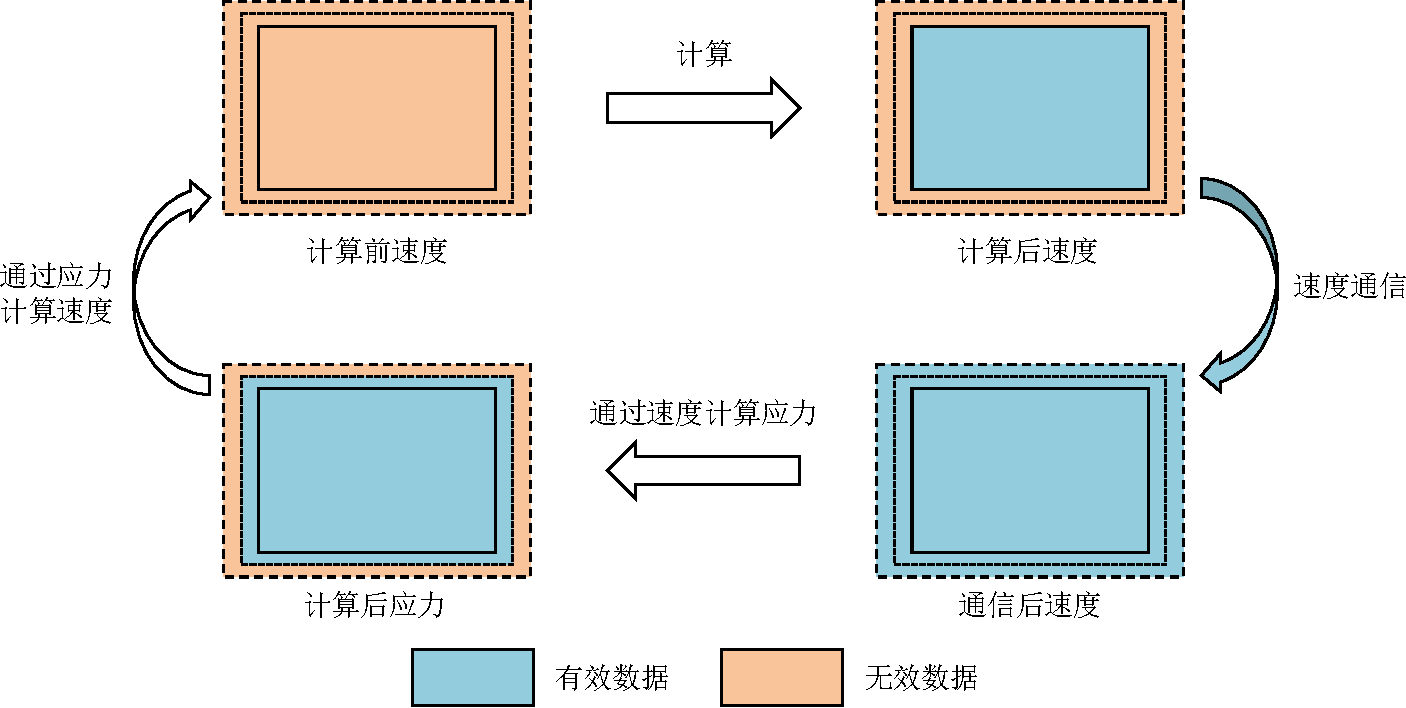
\includegraphics[width=0.9\textwidth]{ghost-cell-crop.pdf}
  \caption{通信缩减过程:使用额外的两层边界对速度网格进行扩展,使用(-3:nx+4, -3:ny+4, 1:NZ)的速度子区域更新应力,然后使用(-3:nx+4, -3:ny+4, 1:NZ)的应力子区域更新速度。额外扩展虚拟网格后,只需进行三个分量的边界通信而无需进行应力六个分量的通信,显著地节约了通信量。}
  \label{fig:ghost-cell}
\end{figure}

本文研究提出的通信缩减方法在已有的两层虚拟网格的基础上额外扩展两层虚拟网格,即共四层虚拟网格(如图\ref{fig:ghost-cell}所示)。以三维速度为例,此时更新区域大小为(1:nx, 1:ny, 1:NZ)的速度子区域需要使用大小为(-3:nx+4, -3:ny+4, 1:NZ)的网格作为输入。进程间需要进行通信的的区域由原来的两层网格变成四层网格。这意味着速度网格通信后有效的区域为(-3:nx+4, -3:ny+4, 1:NZ)。额外的两层边界存储着计算应力需要的内容,这使得应力子区域的更新可以从大小为(-3:nx+4, -3:ny+4, 1:NZ)的速度网格计算得到。另一方面,由于应力网格也是用相同的方法额外扩充两层边界,应力更新后,完整的应力网格可以反过来更新本进程的速度网格,速度和应力的计算通信过程如图\ref{fig:ghost-cell}所示。可以看到,此时只需要对速度网格进行边界通信,无需对应力网格进行通信。在三维弹性波正演算法中,速度包含三个分量,而应力包含六个分量,因此通信量约减少2/3。通信的较少有助于后文介绍的计算通信重叠,更利于在大规模并行时保持良好的扩展性。

虚拟网格技术与计算和通信重叠技术相结合,大规模运行环境下的高效通信效率,在本研究的唐山大地震算例中,取得了接近线性的弱扩展性。

\section{大规模并行IO优化方案}

当并行的规模逐渐增大时,IO将与通信一样逐渐成为整体应用的瓶颈。通信和IO都是为了保证程序的正确运行,此外,IO操作还承担着另外一项重要的功能,通过磁盘保存程序状态。

大规模的地震模拟伴随着巨大的计算量,即便拥有大型超算的支持,计算时间仍然可能需要十几个小时甚至几十个小时。更多计算核心的参与也意味着发生硬件和软件错误的概率更大。重启模块的设计正是为了解决这个问题,但在重启模块的过程中,十六万进程需要分别将进程的内部状态变量输出到网络硬盘中,在没有优化的情况下,这几乎是不可实现的。为了实现大规模的平滑IO操作,本文提出了IO分组、平衡IO和LZ4压缩组合策略。

\subsection{MPI-IO与多进程串行IO}

在大规模地震模拟中,作为输入的介质模型和震源的数据也逐渐增大达到了几十TB量级。在地震模拟初始化时,所有的进程需要分别从磁盘中读取介质模型和震源所对应的部分。此外,在地震模拟的过程中需要间隔一定时间输出波场快照或者地震记录,输出文件大小也在几百GB量级。在大规模并行环境下,通常有两种并行IO的方式:MPI-IO和多进程串行IO。

MPI-IO是MPI标准的补充提供的并行IO接口,支持多个进程共同划分同一个完整的大文件。对于规整的访问模式,MPI-IO通常能够获得很好的性能。本研究的大规模地震模拟使用了规整的介质网格,每个进程读取规整网格的子区域。依赖MPI-IO高性能库,每个进程通过定义文件视图,可以方面读取该进程所需的文件内容,即时这部分内容在文件中并不是连续存储的。

MPI-IO接口适用于传统的Intel、IBM或Cray处理器,因为MPI-IO都在这些处理器上进行了深度的优化,然而MPI-IO并不适合神威超算。神威超算目前并未对MPI-IO进行深入从核优化,MPI-IO性能在神威超算上并不理想,因此本研究使用另外一种更利于神威超算的并行IO策略——多进程串行IO。

多进程串行IO的基本思想是每个进程分别调用朴素的C/C++输入输入接口(如fread, fwrite)执行IO操作。多进程共同发起的串行IO能够充分利用文件系统代理,在块大小(block size)达到256字节时,通常能够获得很好的性能。不过,为了配合多进程串行IO方案,通常需要对完整大文件进行预处理或者后处理操作。例如,在读取介质模型时,首先对介质模型进行预处理,将完整的介质模型根据当前的MPI划分分割成若干小文件,然后每个进程读取对应的小文件。

\subsection{IO分组和平衡IO}

神威超算使用Lustre分布式文件系统,每个节点无本地磁盘。当多进程发起IO请求时,文件系统代理负责处理请求,并将IO数据写入/读取到不同的磁盘。当进程数量达到上万甚至十万量级时,文件系统代理同时处理大量的IO请求效率很低。此外,神威超算文件系统的每个目录文件数量超过10,000时,也同样影响IO效率。本文提出IO分组策略。当160,000进程同时发起IO请求时,将进程分成若干组,每组约5,000个进程,并将IO请求分散到不同的文件系统目录。IO分组能有效降低文件系统代理的压力,降低调度开销,提高效率。

在IO分组的基础上,本文工作提出了平衡IO策略。平衡IO策略的目的是最大化利用文件系统的带宽,包含两部分:(1)发挥所有文件系统代理服务调度效率;(2)使用分条技术将大文件分散到不同物理硬盘。在进行IO分组时,首先确立分组数(如50组),然后使用取模运算将进程号为$0,50,100,150,\ldots$编为第一组,进程号为$1,51,101,151,\ldots$编为第二组,如此类推。这种分组方式中,每一组的进程平均分散到不同的节点和IO代理,能避免IO代理间负载不均衡现象。对于大文件(100+TB)则使用分条技术将文件分散到不同的物理硬盘,或者将大文件划分成若干小文件,并分散到不同物理硬盘中。执行IO操作时,能发挥所有硬盘的带宽。


\subsection{LZ4压缩}

地震模拟的输出来自于三方面:波场快照、地震记录和重启模块。地震模拟的输出有以下特点:
\begin{itemize}
  \item 输出量大:大规模的波场快照和地震记录的输出文件大小通常在几百GB到几十TB数量级;重启模块的输出文件大小非常大,约几百TB;
  \item 含零元素多:根据地震波模拟的特性,在地震波未扩散到完整的地震模拟区域时,波场中有大量的零元素。地震记录也有类似的情景,在信号接收器未收到地震反射信号时,地震记录的值为零。
\end{itemize}

结合上述两个特点,本文研究使用了LZ4压缩方法对波场快照、地震记录和重启文件进行压缩,能有效降低输出文件大小,节约IO带宽和存储空间。

\section{本章小结}

本章对大规模科学应用扩展到神威超算全机时遇到的挑战提出相应的解决方法,,分别从三个方面进行描述:多层级并行任务划分、大规模通信优化和IO优化。多层级并行任务划分方案灵活根据不同计算单元的特性,将完整的计算区域和计算任务分配到不同的计算单元,最大化不同计算单元的性能。大规模通信优化介绍了两种通信优化方法:通过计算通信重叠隐藏通信时间和使用虚拟网格降低通信总量。最后本章介绍了神威超算下的大规模IO优化方法,用多进程串行IO方式替代MPI-IO方式,然后对进程进行IO分组和平衡IO,最后结合地震数据的特征使用LZ4压缩方案降低输出文件大小,节约IO带宽和存储空间。

% chapter 面向神威超算系统的大规模并行优化方法 (end)